% Copyright (c)  2005-2010 EDF-EADS-PHIMECA.
% Permission is granted to copy, distribute and/or modify this document
% under the terms of the GNU Free Documentation License, Version 1.2
% or any later version published by the Free Software Foundation;
% with no Invariant Sections, no Front-Cover Texts, and no Back-Cover
% Texts.  A copy of the license is included in the section entitled "GNU
% Free Documentation License".
\renewcommand{\filename}{docUC_InputNoData_TruncatedDist.tex}
\renewcommand{\filetitle}{UC : Creation of a truncated distribution}

% \HeaderNNIILevel
% \HeaderIILevel
\HeaderIIILevel
\label{truncatedistribution}




\index{Usual Distribution!Truncated distribution}

The objective of the Use Case is to truncate a 1D distribution already defined. Open TURNS enables to truncate the distribution in its lower area, or its upper area or in both lower and upper areas. After having  truncated a distribution, it is possible to recuperate the initial distribution thanks to the method {\itshape getDistribution()}.\\

Details on each object may be found in the User Manual  (\href{OpenTURNS_UserManual_TUI.pdf}{see User Manual - Probabilistic modeling / Truncated Distributions}).\\

Let's consider $X$ a random variable with respectively $F_X$ and $p_X$ its cumulative and probability density functions, and $(a,b)\in \mathbb{R} \cup {\pm \infty}$. The random variable $Y=X/[a,b]$ which is the random variable $X$ given that $X\in[a,b]$ is defined by the following cumulative and probability density functions $F_Y$ and $p_Y$ :
$$
\forall y \in \mathbb{R}, F_Y(y) = Prob(X<y\, / \, X\in[a,b]) =
\begin{array}{|ll}
  1 & \mbox{for } y \geq b, \\
  0 & \mbox{for } y \leq a, \\
  \displaystyle \frac{F_X(y) - F_X(a)}{F_X(b) - F_X(a)} & \mbox{for } y\in[a,b]
\end{array}
$$
$$
\forall y \in \mathbb{R}, p_Y(y) =
\begin{array}{|ll}
  0 &  \mbox{for } y \geq b  \mbox{ or }  y \leq a\\
  \displaystyle \frac{1}{F_X(b) - F_X(a)}\, p_X(y) & \mbox{for } y\in[a,b]
\end{array}
$$





\noindent%
\requirements{
  \begin{description}
  \item[$\bullet$] some lower and upper bounds : {\itshape myLowerBound, myUpperBound}
  \item[type:] reals
  \item[$\bullet$] a 1D distribution : {\itshape myEntireDistribution}
  \item[type:] a Distribution which implementation is UsualDistribution or ComposedDistribution or Mixture
  \end{description}
}
{
  \begin{description}
  \item[$\bullet$] a distribution : {\itshape myTruncatedDistribution}
  \item[type:]  a TruncatedDistribution
  \end{description}
}

\textspace\\
Python script for this UseCase :

\begin{lstlisting}

  # CASE 1 : Truncate the distribution within the range $[myLowerBound, myUpperBound]$
  myTruncatedDistribution = TruncatedDistribution(myEntireDistribution, myLowerBound, myUpperBound)


  # CASE 2 : Truncate the distribution within the range $[myLowerBound, \infty[$ or $[myLowerBound, max[$ if
  # myEntireDistribution was already bounded by $max$
  myTruncatedDistribution = TruncatedDistribution(myEntireDistribution, myLowerBound, TruncatedDistribution.LOWER)


  # CASE 3 : Truncate the distribution within the range $[-\infty, myUpperBound[$ or $[min, myUpperBound[$ if
  # myEntireDistribution was already bounded by $min$
  myTruncatedDistribution = TruncatedDistribution(myEntireDistribution, myUpperBound, TruncatedDistribution.UPPER)

  # Recuperate the initial distribution
  initialDistribution = myTruncatedDistribution.getDistribution()
\end{lstlisting}

\textspace\\

Figures \ref{truncatedDistribution_pdf} and \ref{truncatedDistribution_cdf} show the PDF and CDF of the truncated distributions of a Logistic($\alpha = 1.0$, $\beta  =2.0$) respectively within the ranges $[4.0, \infty[$,  $[-2.0, 5.0]$ and $[-\infty, 3.0]$.

\begin{figure}[H]
  \begin{center}
    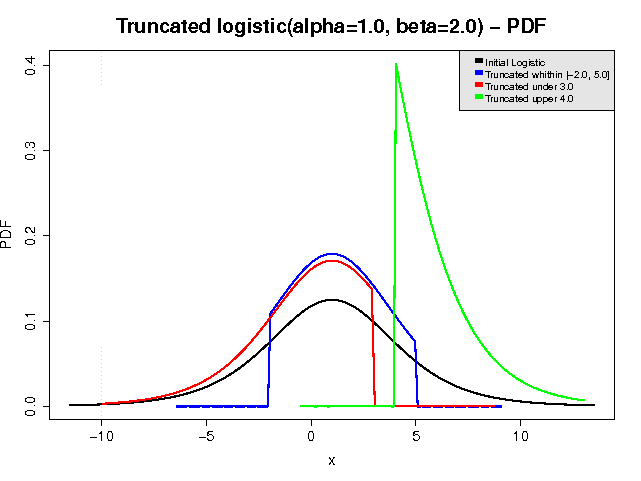
\includegraphics[width=10cm]{truncatedDistribution_pdf.png}
  \end{center}
  \caption{PDF of several truncated Logistic distributions}
  \label{truncatedDistribution_pdf}
\end{figure}

\begin{figure}[H]
  \begin{center}
    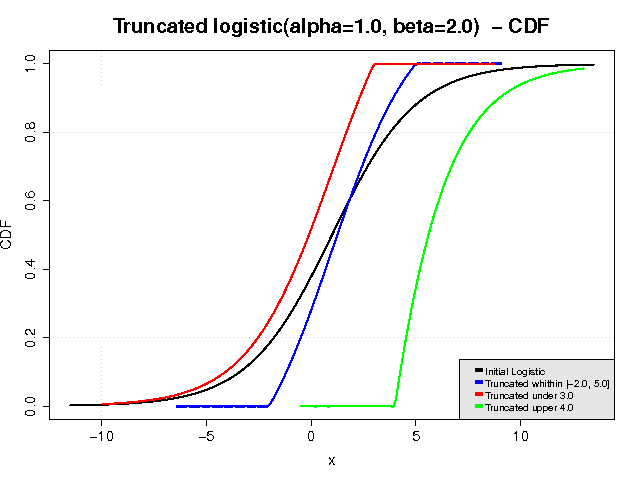
\includegraphics[width=10cm]{truncatedDistribution_cdf.png}
  \end{center}
  \caption{CDF of several truncated Logistic distributions}
  \label{truncatedDistribution_cdf}
\end{figure}

